%section{File Transfers}

\subsection{WLCG data transfers}

For more than the last two years, since we started encouraging the Tier-2 transition, we have been regularly tracking the fraction of WLCG data transfers that take place over IPv6. We have been able to use the IPv6 protocol filter in the monitoring of the total WLCG FTS data transfers.
The fraction of WLCG FTS data transfers over IPv6 as a function of date is shown in  figure~\ref{fig:FTS}.
\begin{figure}[h]
\centering
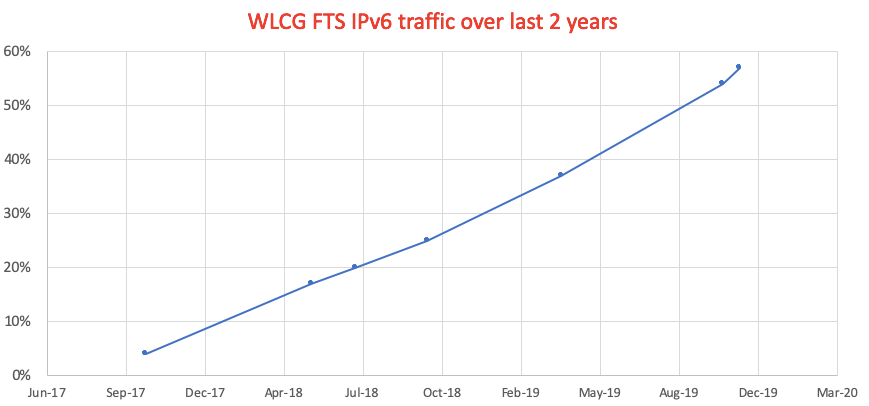
\includegraphics[width=10cm]{FTS}
\caption{Percentage of FTS data transfers over IPv6. Each data point shows the average percentage over the previous 30 days}
\label{fig:FTS}
\end{figure}

We have, from time to time, either observed, or been made aware of, the fact that data transfers between two specific systems have been taking place over IPv4 in spite of the fact that both ends have been dual-stack enabled. We have identified several different reasons why the transfer did not use IPv6, the preferred protocol, and in the majority of cases this has turned out to be due to configuration settings which have either deliberately been set to prefer IPv4 or had been defined that way by mistake. We note that when transfers do take place over IPv6, they do so in such a way that the LHC experiments do not notice any difference in behaviour. We have not received any complaints that data transfers over IPv6 are performing slower or less efficiently than IPv4.